\documentclass[11pt,a4paper]{article}
\usepackage[utf8]{inputenc}
\usepackage[T1]{fontenc}
\usepackage[spanish,es-tabla,es-noshorthands]{babel}
\usepackage[margin=2.3cm]{geometry}
\usepackage{amsmath,amssymb}
\usepackage{graphicx}
\usepackage{booktabs}
\usepackage{float}
\usepackage[hidelinks]{hyperref}

\title{Laboratorio 4: RL\\\large DS5345 -- UTEC}
\author{Jeffrey Monja Castro} % <- cambiar

\begin{document}
\maketitle

\noindent\textbf{Código:} \url{https://github.com/jeffreymonjacastro/rl_lab4}\\


\section{Formulación del MDP}
El entorno implementa un MDP continuo para un TurtleBot3 \emph{burger} en ROS~2 Humble y Gazebo Classic. En el escenario \emph{cruce}, la meta permanece en $(1.5,0)$~m. Dos obstáculos móviles atraviesan la ruta y reciben una fase inicial aleatoria en cada reinicio.

\paragraph{Estado ($s_t \in \mathbb{R}^{52}$).} La observación concatena 24 distancias LiDAR mínimas por sector, normalizadas por $3.5$~m, y 24 velocidades de cierre estimadas a partir de barridos consecutivos. Estas velocidades compensan la rotación del robot, se limitan a $\pm1.5$~m/s y se normalizan por $1.5$. También incluye las velocidades lineal y angular de la odometría, normalizadas por sus máximos; la distancia a la meta en metros; y el ángulo relativo a la meta dividido entre $\pi$.

\paragraph{Acción continua.} La acción $a_t=(v_t,\omega_t)$ se envía como un mensaje \texttt{Twist} por \texttt{/cmd\_vel}. El entorno limita $v_t$ a $[0,0.22]$~m/s y $\omega_t$ a $[-2.84,2.84]$~rad/s. Cada paso avanza la simulación durante $\Delta t=0.2$~s.

\paragraph{Recompensa y fin del episodio.} Si $d_t$ es la distancia actual a la meta, la recompensa se calcula como
\[
    r_t = \frac{1}{\max(d_t,0.20)^2} - 10 I_{\text{choque}} + 10 I_{\text{meta}}.
\]
Hay choque cuando la lectura LiDAR mínima baja de $0.15$~m. Se alcanza la meta cuando $d_t<0.20$~m y no hay choque. Si no ocurre ninguno de estos casos, el episodio se trunca al llegar al límite predeterminado de 150 pasos.

\section{Parte A: A2C y PPO}
Ambos métodos usan la misma arquitectura (actor $52\to128\to128\to2$ y crítico $V(s)$), rollouts de 64 pasos y GAE con $\gamma=0.99$ y $\lambda=0.95$. Se entrenaron durante 20\,000 pasos; PPO usa recorte $L^{CLIP}$ con $\epsilon=0.2$, cuatro épocas por actualización y parada si la KL supera 0.03.

\begin{figure}[H]
    \centering
    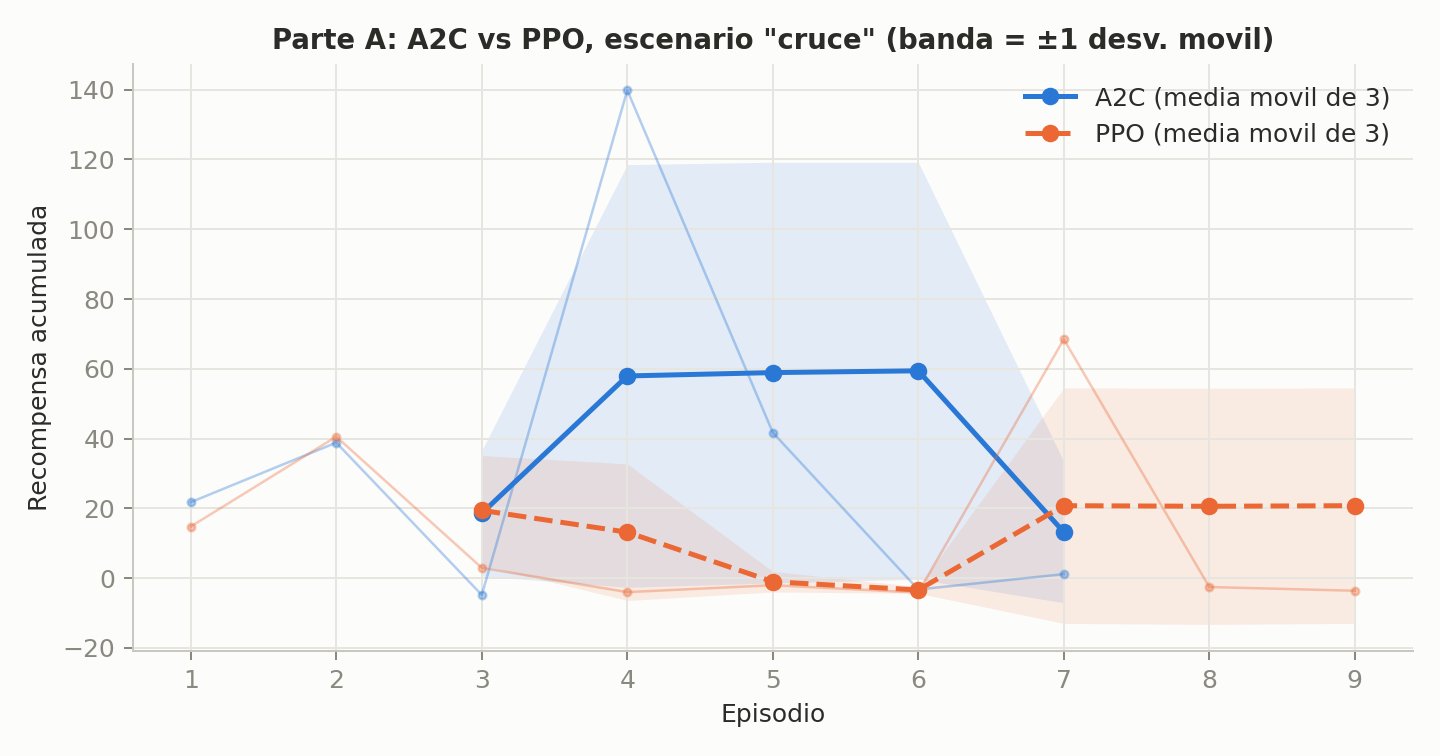
\includegraphics[width=0.85\linewidth]{report/A/recompensa_a2c_vs_ppo.png}
    \caption{Recompensa por episodio en el escenario \emph{cruce}. Las curvas muestran una media móvil de tres episodios y la banda indica $\pm1$ desviación estándar.}
\end{figure}

En esta corrida corta, A2C alcanza una media móvil cercana a 60 entre los episodios 4 y 6, pero cae después y presenta mayor variación. PPO baja cerca de cero a mitad del tramo; luego se recupera hasta aproximadamente 20 y se mantiene allí en los episodios mostrados. La cantidad reducida de episodios y la amplitud de las bandas hacen que esta comparación sea descriptiva, no concluyente.

\begin{figure}[H]
    \centering
    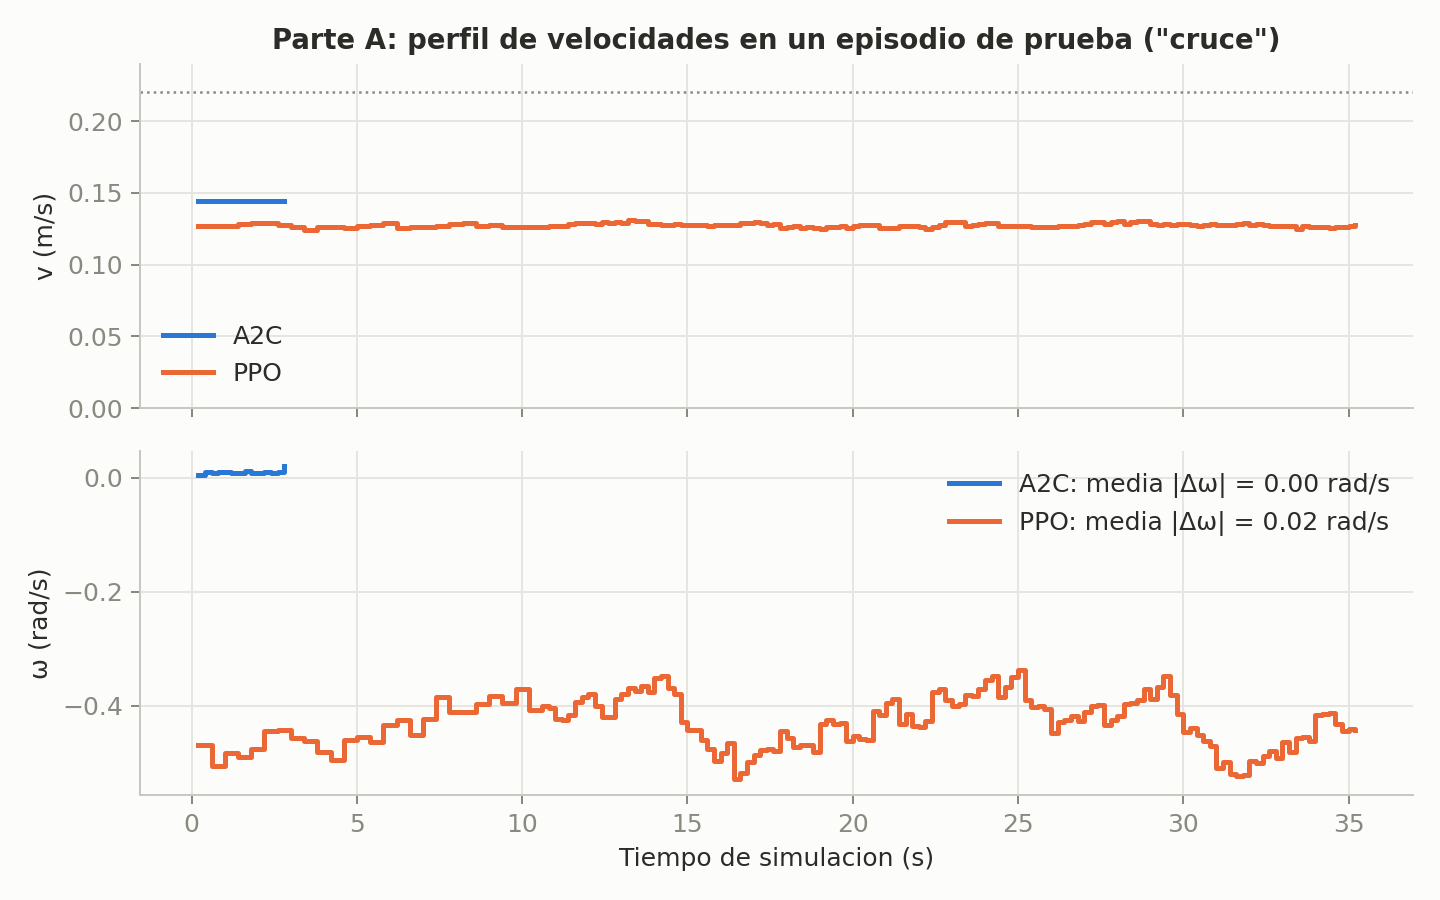
\includegraphics[width=0.8\linewidth]{report/A/velocidades_a2c_vs_ppo.png}
    \caption{Velocidades lineal $v$ y angular $\omega$ registradas en un episodio de prueba del escenario \emph{cruce}.}
\end{figure}

En el episodio representado, PPO avanza alrededor de $0.13$~m/s y gira principalmente hacia valores negativos de $\omega$; A2C conserva una velocidad lineal algo mayor y una velocidad angular cercana a cero. La figura reporta un cambio medio de $|\Delta\omega|$ de $0.00$~rad/s para A2C y $0.02$~rad/s para PPO. Es un único episodio, por lo que no basta para caracterizar la suavidad general de ambas políticas.

\section{Parte B: Imitación del comportamiento frente a DAgger}


\section{Parte C: RLHF y pruebas de estrés}


\section{Conclusiones}

\begin{itemize}
    \item 1
\end{itemize}

\end{document}
